%% Based on a TeXnicCenter-Template by Gyorgy SZEIDL.
%%%%%%%%%%%%%%%%%%%%%%%%%%%%%%%%%%%%%%%%%%%%%%%%%%%%%%%%%%%%%

%----------------------------------------------------------
%
\documentclass[a4paper, twoside, final]{book}%
\usepackage{amsmath}%
\usepackage{amsfonts}%
\usepackage{amssymb}%
\usepackage{graphicx}
\usepackage{url}
\usepackage{listings}
\usepackage{color}
\usepackage{wrapfig}
\usepackage{subfig}
\usepackage{float}
\usepackage{hyperref}
\usepackage[T1]{fontenc}
\usepackage[utf8]{inputenc}
\definecolor{Grey}{rgb}{0.85,0.85,0.85} 
\lstset{language=C, backgroundcolor=\color{Grey}}
%----------------------------------------------------------
\newtheorem{theorem}{Theorem}
\newtheorem{acknowledgement}[theorem]{Acknowledgement}
\newtheorem{algorithm}[theorem]{Algorithm}
\newtheorem{axiom}[theorem]{Axiom}
\newtheorem{case}[theorem]{Case}
\newtheorem{claim}[theorem]{Claim}
\newtheorem{conclusion}[theorem]{Conclusion}
\newtheorem{condition}[theorem]{Condition}
\newtheorem{conjecture}[theorem]{Conjecture}
\newtheorem{corollary}[theorem]{Corollary}
\newtheorem{criterion}[theorem]{Criterion}
\newtheorem{definition}[theorem]{Definition}
\newtheorem{example}[theorem]{Example}
\newtheorem{exercise}[theorem]{Exercise}
\newtheorem{lemma}[theorem]{Lemma}
\newtheorem{notation}[theorem]{Notation}
\newtheorem{problem}[theorem]{Problem}
\newtheorem{proposition}[theorem]{Proposition}
\newtheorem{remark}[theorem]{Remark}
\newtheorem{solution}[theorem]{Solution}
\newtheorem{summary}[theorem]{Summary}
\newenvironment{proof}[1][Proof]{\textbf{#1.} }{\ \rule{0.5em}{0.5em}}
%----------------------------------------------------------
\begin{document}

\frontmatter
\title{The Rolling Pins \\ Developers Guide}
\author{Arnþór Magnússon}
\date{1. Version, October 2012}
\maketitle
\tableofcontents

\part{Getting Started}

\chapter{Introduction}
The Rolling Pins are modular robotic devices, that can output light in different colors, vibration and audio. They can be interacted through movement (accelerometer and gyroscope), other pins and other devices containing wireless module.

\begin{figure}[H]
  \centering
  \begin{tabular}{cc}
    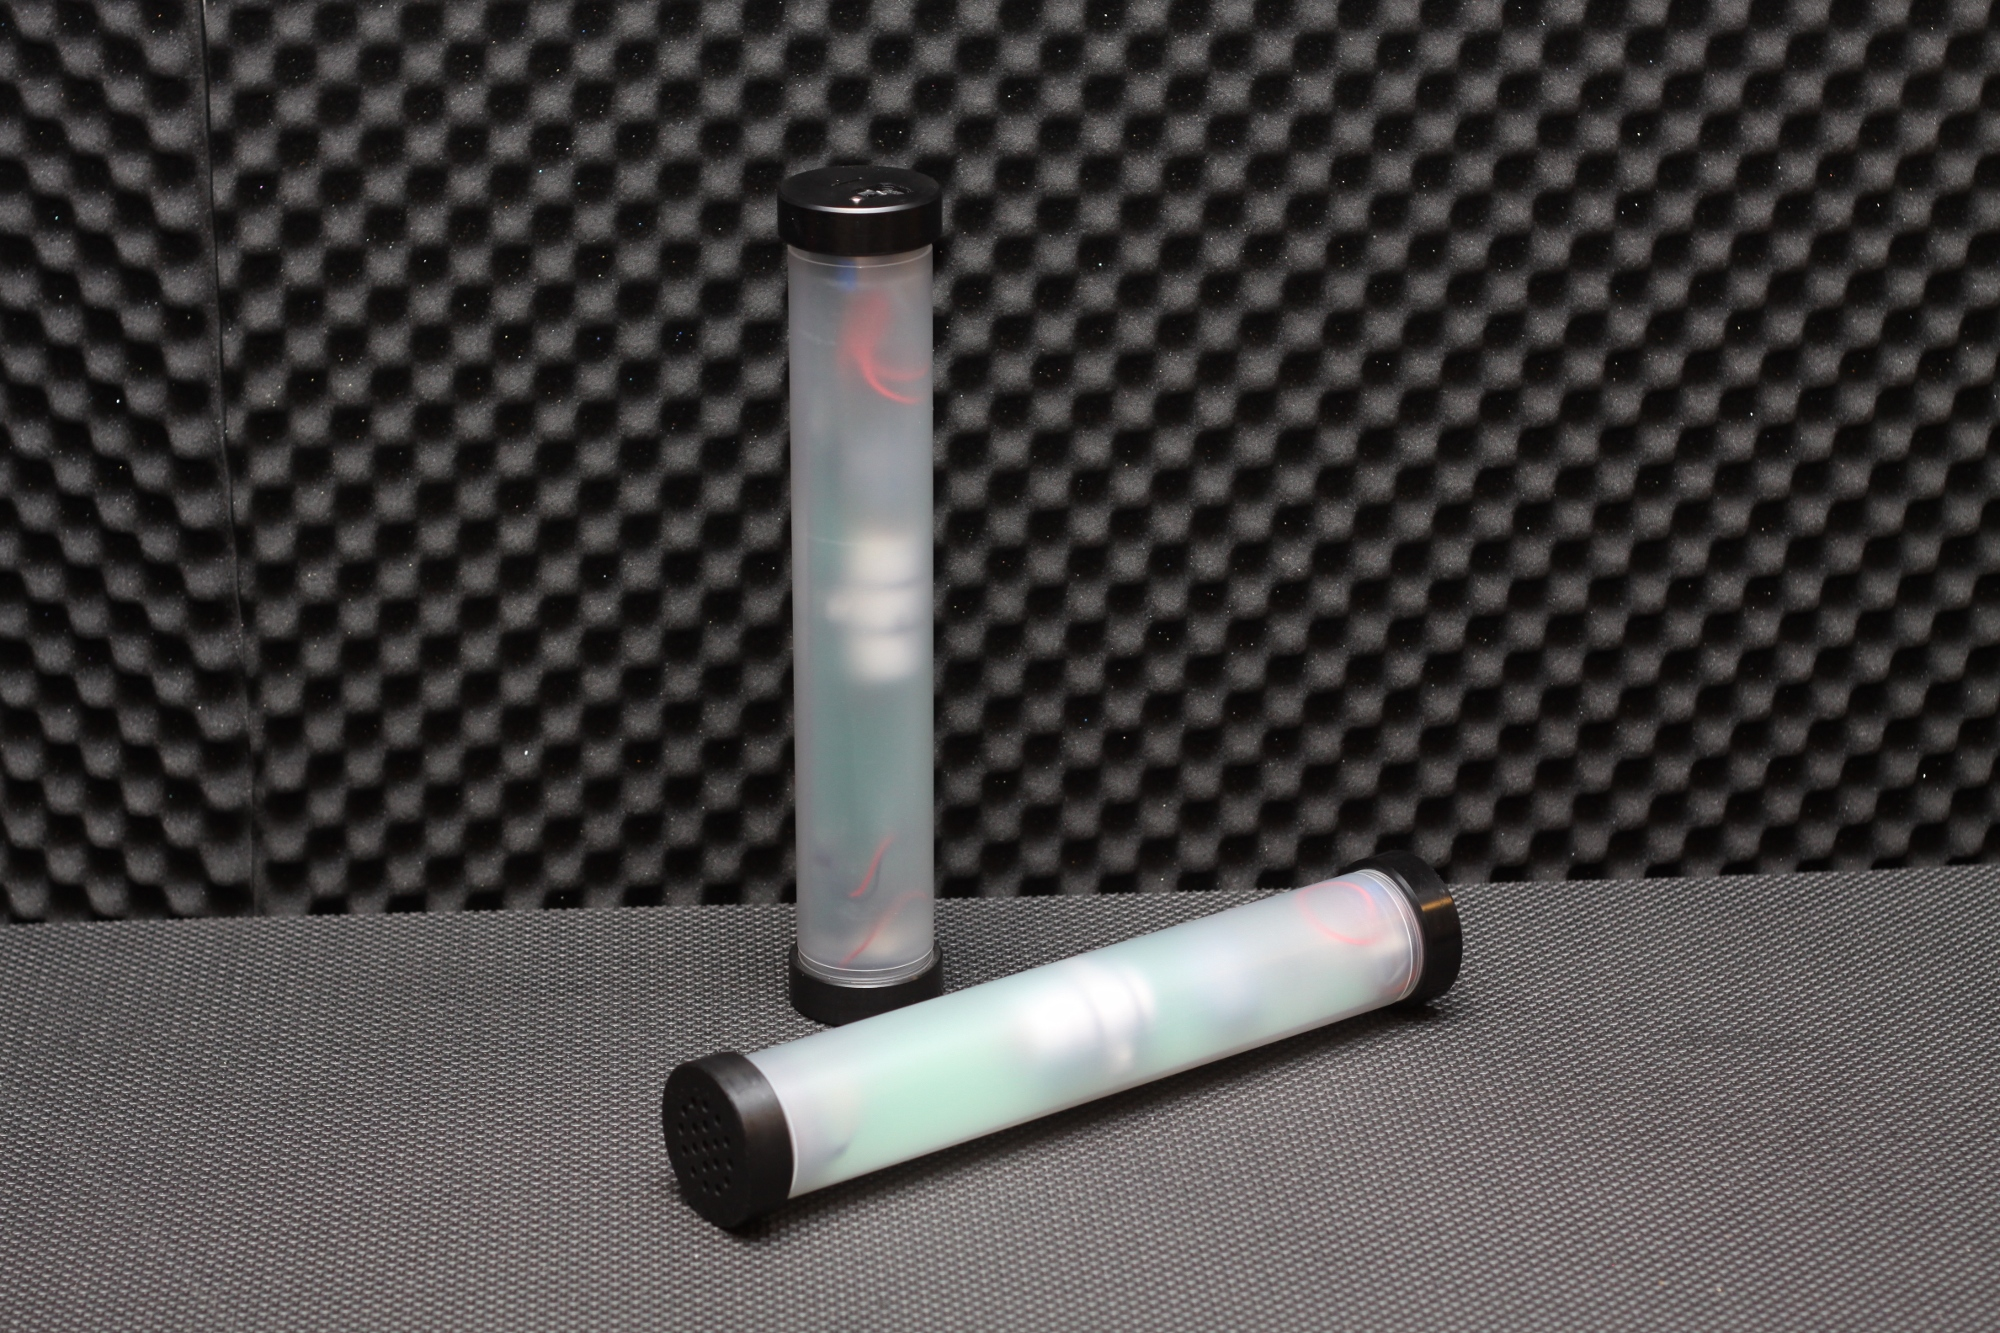
\includegraphics[width=0.5\textwidth]{figures/pins.JPG}
    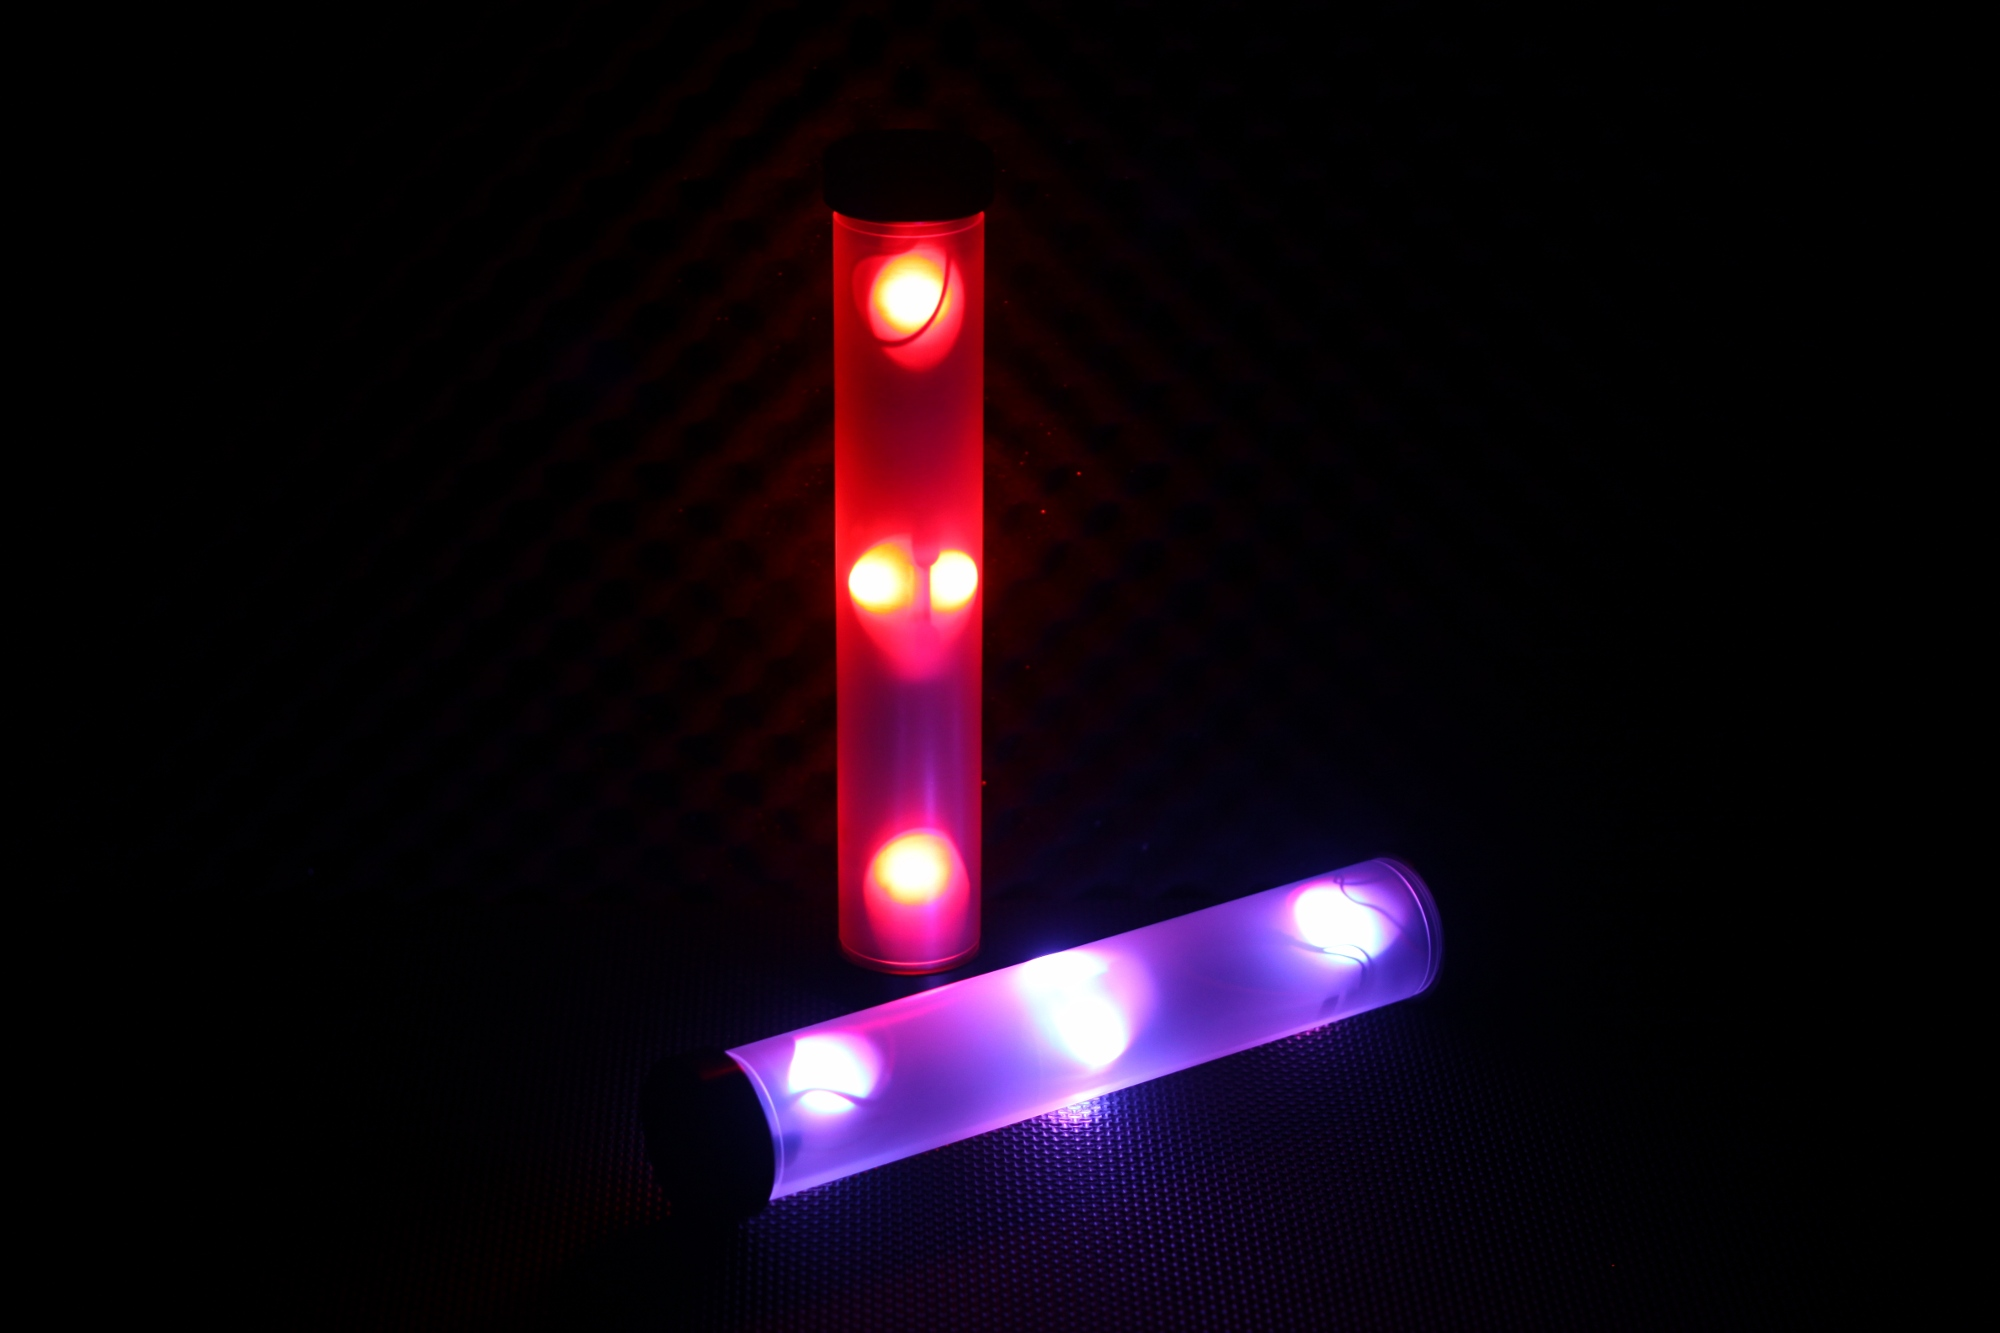
\includegraphics[width=0.5\textwidth]{figures/pins_lights.JPG} &
  \end{tabular}
  \caption{The Rolling Pins.}
  \label{fig:rollingpins}
\end{figure}

The Rolling Pins are made out of sturdy translucent plastic material which forms a cylinder. A black lid is screwed on each end of the cylinder, the top end contains the power connector and the JTAG programming connector, while the bottom end contains the speaker. 

\subsection*{Internal hardware}
\begin{itemize}
\item	One 8bit RISC Atmel ATMega 1280 processor.
\item	Eight RGB LEDs \\
Each with 16 levels of intensity per color, thus able to display up to 4096 different colors.
\item One vibrator.
\item One Speaker and a audio module.\\
Audio can be played from a SD memory card through a speaker.
\item One accelerometer and a gyroscope.\\
To measure movement and orientation of the pin.
\item One XBee communication chip. \\
The XBee allows for communication between pins, as well as other devices containing XBee modules.
\end{itemize}

\mainmatter

\chapter{Software Installation}

This chapter describes the useful and in most cases necessary software installations for developing applications for the Rolling pins. We recommend setting up all the following software:

\section{Source code}

\section{Windows Installation (32bit)}
\label{windows_installation_32bit}

\subsection*{Source Code}
The source code for the pins is located at Github: \url{https://github.com/Playware/Pins}.
To download the code, one must have a Git client, one such is TortioiseGit:

\begin{enumerate}
  \item Download a Git client and install, TortioiseGit:\\
    \url{http://code.google.com/p/tortoisegit/}
  \item Create a new folder that is supposed to contain the source code.
  \item Right click on the new folder and select TortioiseGit->Clone
    and enter the Github url: \url{https://github.com/Playware/Pins},
    continue and the program fetches the source code and places it in the folder.
\end{enumerate}

\subsection*{X-CTU Software (optional)}
X-CTU is a stand-alone tool for configuring XBee modules.
\begin{enumerate}
	\item Download the installation file from:\\ 
	\url{ftp://ftp1.digi.com/support/utilities/Setup_XCTU_5260.exe}
	\item Browse to where the file is stored.
	\item Double-click on the installer file and follow the X-CTU Setup Wizard.
	\item When asked if you would like to check Digi's website for firmware updates, click Yes. 
	\item After the firmware updates are complete, click Close.
	\item Start X-CTU by double-clicking on the X-CTU icon placed on your desktop or by selecting: 
Start $>$ Programs $>$ Digi $>$ X-CTU 
\end{enumerate}

\subsection*{\bf FTDI Driver for XBEE}
In many cases this driver will be installed automatically when the XBee module is plugged into a windows computer. If not, follow these steps:
\begin{enumerate}
	\item Download the installation file from: \\ 	   
	Win98 - XP: \url{http://ftp1.digi.com/support/driver/40002636_A.zip}
	Vista/Win7: \url{ftp://ftp1.digi.com/support/driver/ftdi_WindowsVista_7_Drivers.zip}
	\item Unzip the file to a folder and point the windows driver installation to look for the driver in that folder.
	\item Windows should set up the driver automatically from there	
\end{enumerate}

\subsection*{\bf Atmel AVR Studio (optional)}
The Atmel AVR Studio is a great tool for JTAGing and debugging. It also includes the driver for the JTAG ICE MkII programmer/debugger used at Center For Playware.
\begin{enumerate}
	\item Download version 4 of the program and all service packs if available from: \\
	\url{http://www.atmel.com/dyn/products/tools_card.asp?tool_id=2725}\\
or version 5 from: \\
\url{http://www.atmel.com/dyn/products/tools_card.asp?tool_id=17212&source=avr_5_studio_overview}\\
In both cases a registration might be required.	
	\item Install the program and all service packs in order by running the executable files.
\end{enumerate}

\subsection*{\bf Win AVR (AVR GCC) Compiler Suite}

The Win AVR Compiler Suite includes the avr gcc compiler needed for compiling code for the pins from Eclipse.
\begin{enumerate}
	\item Download the latest version of the program from: \\
	\url{http://sourceforge.net/projects/winavr/files/WinAVR/}
	\item Double click the installer file and follow the wizard.
\end{enumerate}

\subsection*{\bf Eclipse (Eclipse IDE for C/C++ Developers) (32-bit) (optional)}
Eclipse is a Java based programming environment which has proven to be very good for creating C code.
\begin{enumerate}
	\item Download the latest version of the C/C++ version of the program from: \\
	\url{http://www.eclipse.org/downloads/}
	\item Unzip the file to a desired folder (No installation required).
\end{enumerate}

\subsection*{\bf AVR GCC Plugin for Eclipse (optional)}
AVR GCC Plugin is necessary for compiling software through Eclipse
\begin{itemize}
	\item See further instructions following the link: \\
	\url{http://avr-eclipse.sourceforge.net/wiki/index.php/Plugin_Download}
\end{itemize}

\subsection*{\bf Arduino environment}
The Rolling Pins uses the Arduino framework for convenience. 
\begin{enumerate}
  \item Download the latest version of the program from: \\
  \url{http://arduino.cc/en/Main/Software}
  \item Unzip the downloaded file when it finishes, make sure to preserve the folder structure
\end{enumerate}

\newpage

\section{Linux Installation}

%\subsection*{\bf FTDI Driver for XBEE}
%FTDI drivers are built in since kernel 2.6.9 and greater.

\subsection*{Source Code}
The source code for the pins is located at Github: \url{https://github.com/Playware/Pins}.
To download the code, one must have a Git client, which is available in the Linux package manager.

\begin{enumerate}
  \item To get Git, open a terminal and type:\\
\begin{lstlisting}
apt-get install git
\end{lstlisting}
  \item Go to a directory you want to place the source code:
    \begin{lstlisting}
cd /path/to/source/code/
    \end{lstlisting}
  \item Pull the source code from Github:\\
    \begin{lstlisting}
git clone https://github.com/Playware/Pins
    \end{lstlisting}
\end{enumerate}

\subsection*{\bf AVR Libc and AVR-GCC compiler}
AVR-GCC and Libc are required in order to develop and compile the source for the AVR microchip. 
In many cases this software can be installed from a package manager within your Linux distribution. For example in Debian based distro:

\begin{lstlisting}
  apt-get install gcc-avr avr-libc
\end{lstlisting}

Otherwise the software is available at \url{http://www.nongnu.org/avr-libc/}.

\subsection*{\bf Eclipse (Eclipse IDE for C/C++ Developers) (optional)}
Eclipse is a Java based programming environment which has proven to be very good for creating C code.
\begin{itemize}
  \item Install via package manager:
\begin{lstlisting}
  apt-get install eclipse-cdt
\end{lstlisting}
\end{itemize}
or
\begin{enumerate}
	\item Download the latest version of the C/C++ version of the program from: \\
	\url{http://www.eclipse.org/downloads/}
	\item Unpack program and run eclipse.
\end{enumerate}

\subsection*{\bf AVR GCC Plugin for Eclipse (optional)}
AVR GCC Plugin is necessary for compiling software through Eclipse
\begin{itemize}
	\item See further instructions following the link: \\
	\url{http://avr-eclipse.sourceforge.net/wiki/index.php/Plugin_Download}
\end{itemize}


\subsection*{\bf AVRDude}
\emph{avrdude} is used to upload a compiled program to a individual pin. It can be installed using a package manager:

\begin{lstlisting}
  apt-get install avrdude
\end{lstlisting}
or by visit avrdude webpage \url{http://www.nongnu.org/avrdude/} and follow their instructions.

\subsection*{\bf Arduino environment}
The Rolling Pins uses the Arduino framework for convenience.
\begin{itemize}
  \item Install via package manager:
\begin{lstlisting}
  apt-get install arduino
\end{lstlisting}
\end{itemize}
or 
\begin{enumerate}
  \item Download the latest version of the program from: \\
  \url{http://arduino.cc/en/Main/Software}
  \item Unzip the downloaded file when it finishes, make sure to preserve the folder structure
\end{enumerate}

\newpage

\section{Setup and Configuration}

%In which environment to program the Rolling Pins is a matter of opinion. The author of this document prefers to use \emph{vim} to program and when finished, one connects the Rolling Pin to the JTAG ICE MkII programmer/debugger which in turn is connected to the computer. The code is compiled using the Make build utility which needs to be configured, by setting the path to previously installed Arduino environment in the file {\tt Makefile} at the RollingPins directory. Find the variable ARDUINO_DIR and set it to the Arduino install directory. Then all you need is to go to the RollingPins directory and run the following command in terminal:
In which environment to program the Rolling Pins is a matter of opinion. The author of this document prefers to use \emph{vim} to program and when finished, one connects the Rolling Pin to the JTAG ICE MkII programmer/debugger which in turn is connected to the computer. The code is compiled using the Make build utility which needs to be configured, by setting the path to previously installed Arduino environment in the file {\tt Makefile} at the {\tt RollingPins} directory. Find the variable {\tt ARDUINO\_DIR} and set it to the Arduino install directory. Then all you need is to go to the {\tt RollingPins} directory and run the following command in terminal:

\begin{lstlisting}
  make upload
\end{lstlisting}

and the make script compiles and uploads the program to the pin. The make script is supported by many programming environments and are easily configured to use the provided {\tt Makefile}. If one prefers to use Eclipse environment, it would be wise to follow the instructions in the Tile manual.

\newpage

\section{The Rolling Pin Folder Structure}

The programing framework is divided into several directories depending on functionality.

\begin{itemize}
  \item RollingPins
  \begin{itemize}
    \item \textbf{Controller} {\it (Here you can find various functions for timers, events and communication protocol.)}
    \item \textbf{Drivers} {\it (Here are the drivers for the various modules of the pins such as Light, Speakers, Accelerometer etc.)}
    \item \textbf{Applications} {\it (Here all the applications reside, where each application has it's own folder.)}
    \item \textbf{Libraries} {\it Here you can find the various libraries, for instance for the XBee module.}
    \item \textbf{Bin}
    \item makefile
  \end{itemize}
\end{itemize}

\subsection*{The important files}
The important files that you need to look at are:
\begin{itemize}
  
  \item \textbf{Application.h}\\
  This file resides in the application folder and is a header file with all applications made for the Rolling Pins. The application to be run needs to be defined as the DEFAULT\_APPLICATION. When a new program is made, a new line with an extern Application needs to be added.
  REMEMBER that the name of the application in this file can not be exactly the same as the \emph{namespace} in the application itself.

  \item \textbf{Application.cpp}\\
  This file resides in the application folder and is a container file with all applications made for the Rolling Pins. When a new program is made, the new application needs to be added to the \emph{*apps} array.\\

  \item \textbf{RPApi.h}\\
  This file holds some global configurations and some system functions. It is a good idea to include this file into every application made for convenience. 
  
  \item \textbf{Makefile}\\
  This file is a part of a automatic build system, to build the program into hex file and uploading to a pin. This file might need editing, to set the path to Arduino environment.

  \item \textbf{HelloWorld.cpp}\\
  This file resides in the HelloWorld folder in the application folder and is a template for a new program. When making a program it is best to make a copy of this file and start from there.
  
\end{itemize}

\newpage
\section{Compiling and Uploading Programs to the Pins}

First the code needs to be compiled, which is done using the Make build system, by going into the {\tt RollingPins} directory in a terminal or command line window, and type

\begin{lstlisting}
  make
\end{lstlisting}

which creates a hex file into the {\tt bin} directory.

\begin{figure}[H]
  \centering
  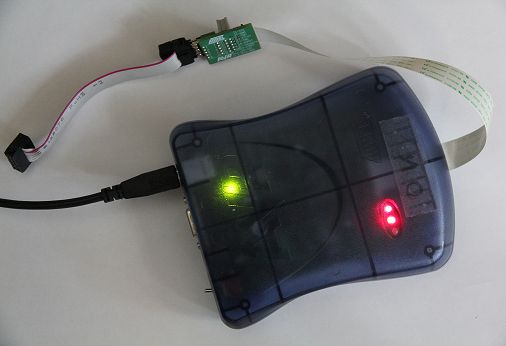
\includegraphics[width=0.6\textwidth]{figures/JTAG_ICE_MkII.png}
  \caption{A JTAG ICE MkII.}
  \label{fig:JTAG_ICE_MkII}
\end{figure}

To upload this program to a pin, a external programmer with JTAG interface is required, such as JTAG ICE MkII (see figure \ref{fig:JTAG_ICE_MkII}). The programmer is plugged both to the computer via USB and to one pin, where the pin is connected with a regular cable directly to the JTAG connector which is located on top of the Rolling Pin, as seen in figure \ref{fig:JTAG_PIN}. 

\begin{figure}[H]
  \centering
  % TODO: Provide new image here:
  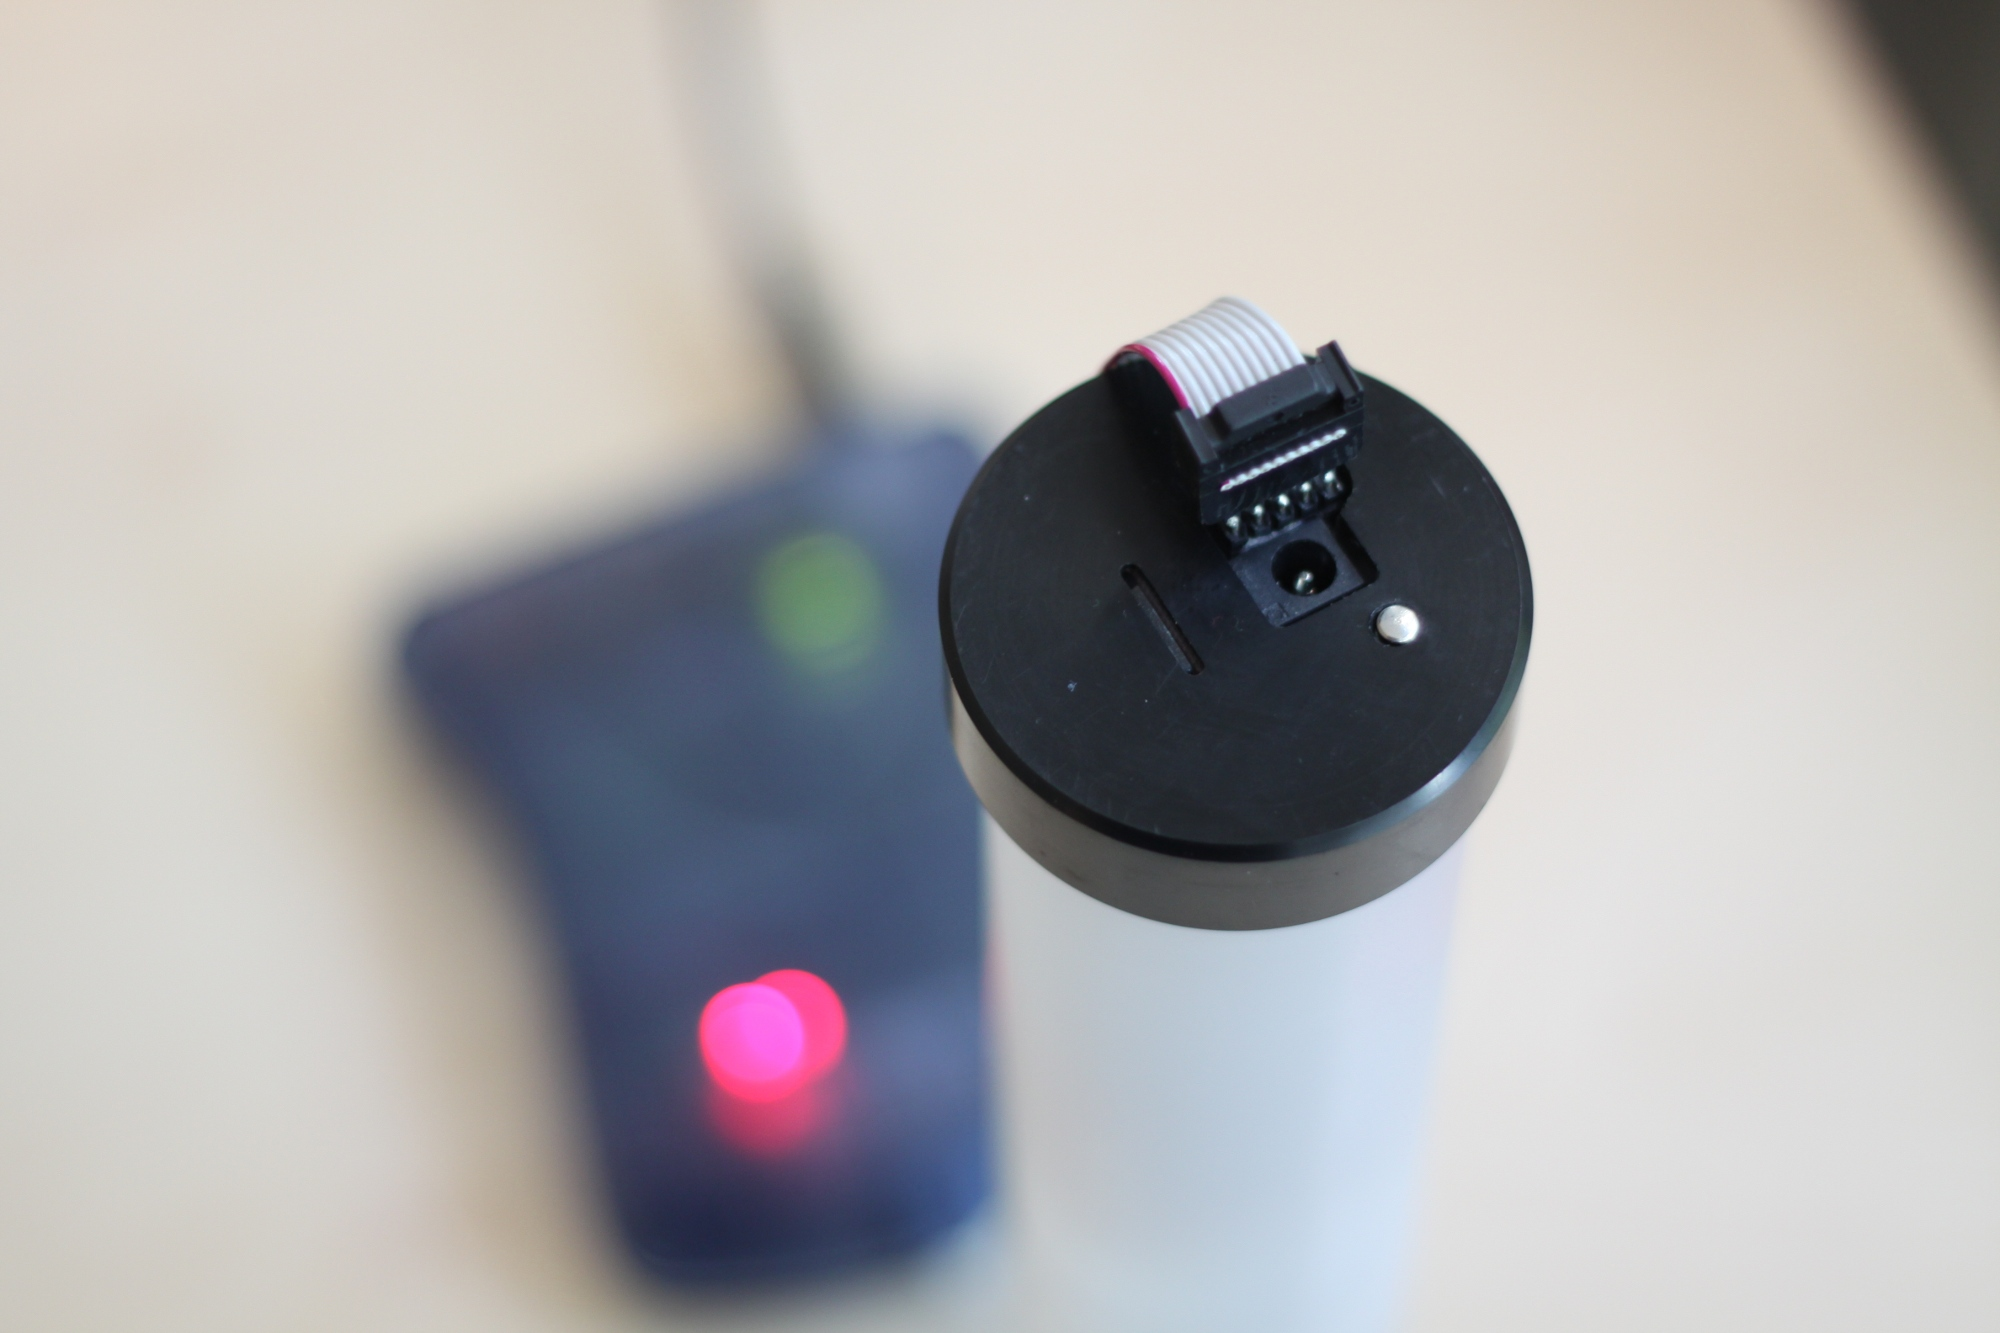
\includegraphics[width=0.6\textwidth]{figures/jtag_connector.jpg}
  \caption{Programmer connected to a pin through the JTAG plug.}
  \label{fig:JTAG_PIN}
\end{figure}

When the program has been compiled it is ready to be uploaded to a pin, which can be done using the command:

\begin{lstlisting}
  make upload
\end{lstlisting}

\part{Programming the Pins}

\chapter{Your First Program}
\section{"Hello World"}
\label{hello_world}

For this example application we will make a pin version of the famous Hello World example. In our case it means that we will turn on all LEDs for the pin for one second and then off again for the same time.\\
\\
First we start creating a directory called \emph{HelloWorld} in the \emph{application} directory and create and open a file called \emph{HelloWorld.cpp}. Then we can fill it with a bare bone application

\begin{lstlisting}
#include "RPApi.h"

namespace HelloWorld
{
  static void setup();
}

Application_t helloWorld = {"HelloWorld", HelloWorld::setup};

static void HelloWorld::setup()
{
}
\end{lstlisting}

First to notice is the declaration of the variable \texttt{helloWorld}

\begin{lstlisting}
Application_t helloWorld = {"HelloWorld", HelloWorld::setup};
\end{lstlisting}

which defines an object containing a reference name for our application \emph{HelloWorld} and a starting point, function called \texttt{setup}.
From the function \texttt{setup()} we can setup the flow of our program, for instance create loops or timers to execute some code with certain intervals or how to handle incoming packets or messages.
For our application we want to create a timer that executes a function we create with 1 sec. interval. Lets call our function \texttt{onTimerFired()}.

\begin{lstlisting}
  static void onTimerFired()
  {
    // Our code will be put here
  }
  
  static void HelloWorld::setup()
  {
    timerManager.createPeriodic(0, 1000, onTimerFired);
  }
\end{lstlisting}

In order to turn on and off all the LEDs we use the functions 

\begin{lstlisting}
  light.setAll(200, 200, 200) // turn on
  light.update()
  // and 
  light.clearAll() // turn off
  light.update()
\end{lstlisting}

where \texttt{setAll(red, green, blue)} sets all LEDs to a color depending on the values given (from 0 to 255), while \texttt{clearAll()} turns all of them off. The \texttt{update()} function needs to be issued every time lights should be changed.
\\
Then we can create some logic to turn on and off our LEDs

\begin{lstlisting}
static bool isOn = false;

static void onTimerFired()
{
  if (isOn)
    light.clearAll();
  else
    light.setAll(LIGHT_WHITE);
  light.update();
  isOn = !isOn;
}
\end{lstlisting}

Next step is to register our new application as a part of the pins software and make it start when the pin is turned on.
To register the application, open the file \emph{Application.h} and add the line 

\begin{lstlisting}
  extern Application_t helloWorld;
\end{lstlisting}

then add \texttt{\&helloWorld} (hint: which was defined in HelloWorld.cpp) to the array \texttt{*apps[]} in \emph{Application.cpp}.
To tell the compiler that we want our application to run at startup, open the file \emph{Application.h} and find the line

\begin{lstlisting}
  #define DEFAULT_APPLICATION &someApplicationName
\end{lstlisting}

and change \texttt{\&someApplicationName} to \texttt{\&helloWord}. 

Finally compile and upload the program to a pin and to see your application in action.

\newpage

\chapter{Digging Deeper}
Now that we have a working program that can be compiled and uploaded to the Rolling Pins, we can start creating more complex code.

\section{The Leds}
Each pin has eight RGB leds with 8 bit resolution per color. That means that you can set the value of each channel between 0 and 255, the higher value the stronger intensity of the color is added to the mix.\\
\\
The functions for manipulating the LEDs should already be included in your application through the \texttt{RPApi.h} file, but are defined in \textbf{drivers/Light.h}. The packet has four functions worth to mention:

\begin{itemize}
  \item \texttt{void setAll(uint8\_t red, utin8\_t green, utin8\_t blue)} \\
	  This function takes in values for the red, green, and blue part of the color and sets that value for all the LEDs.
  \item \texttt{void set(uint8\_t idx, uint8\_t red, utin8\_t green, uint\_t blue)}\\
	  This function takes in values for the red, green, and blue part of the color and sets that value for the corresponding LED (0-7).
  \item \texttt{void clearAll()}\\
    This function turns all LEDs off or more specifically, sets the value for red, green and blue to 0.
  \item \texttt{void update()}\\
    After changing the color of any LED, one must call this function to actually update the changes.
\end{itemize}

\section{Vibrator}
A vibrator is present in each pin, to interact with a user. Three functions can be utilized and are available through the \textbf{RPApi.h} file. There are three function that can manipulate the vibrator:

\begin{itemize}
  \item \texttt{vibrator.on()}\\
    This function turns on the vibrator.
  \item \texttt{vibrator.off()}\\
    This function turn off the vibrator.
  \item \texttt{vibrateUntil(uint16\_t milliSec)}\\
    This function turns the vibrator on for \texttt{milliSec} milliseconds and then off again.
\end{itemize}

\section{Sound}
In order to play a sound or music, a micro-SD memory card must be present in the pin, containing files on the ADPCM (.ad4) format and be named accordingly \textbf{0000.ad4}, \textbf{0001.ad4} \dots \textbf{0511.ad4}.
Wave and MP3 files can be converted to this format using software provided by 4D Systems, which is found at this URL:\\
\url{http://www.4dsystems.com.au/prod.php?id=73}

Functions are provided to play the sound files present on the memory card, these functions are accessed through the \texttt{sound} object that is available through the \textbf{RPApi.h} file.
Below is a list of available functions and their descriptions:

\begin{itemize}
  \item \texttt{play()}\\
    Plays/pauses a song.
  \item \texttt{playSong(uint8\_t idx)}\\
    Starts playing the song with the specified index (\texttt{idx}), the index is a reference to a file on the memory card having a filename containing the index number.
  \item \texttt{stop()}\\
    Stops playing.
  \item \texttt{next()}\\
    Skips to the next sound file with a greater index number.
  \item \texttt{prev()}\\
    Skips to the previous sound file with a smaller index number.
  \item \texttt{setVol(uint8\_t level)}\\
    Sets the volume level, there are 7 levels from 1 to 7.
  \item \texttt{incVol()}\\
    Increases the volume level by one.
  \item \texttt{decVol()}\\
    Decreases the volume level by one.
  \item \texttt{getVol()}\\
    Returns the current volume level.
  \item \texttt{getNowPlaying()}\\
    Returns the current song playing.
  \item \texttt{isPlaying()}\\
    Returns true or false depending if a song is playing.
\end{itemize}


\section{Movement}

Each pin has a accelerometer and a gyroscope that allows to detect movements of 6 degrees of freedom (DoF).
The object \texttt{movement} is available through the \textbf{RPApi.h} file which acts as a interface to the accelerometer and gyroscope, 
the available functions are:

\noindent \textbf{Accelerometer:}\\
The accelerometer values are given in multiples of the gravity ($n\times G$, where $G$ is the acceleration of the gravity).
\begin{itemize}
  \item \texttt{Rx()}\\
    Returns the magnitude of the acceleration in X direction.
  \item \texttt{Ry()}\\
    Returns the magnitude of the acceleration in Y direction.
  \item \texttt{Rz()}\\
    Returns the magnitude of the acceleration in Z direction.
  \item \texttt{R()}\\
    Returns the overall magnitude of the acceleration.
\end{itemize}

\noindent \textbf{Angle position:}\\
The rotation of the pin can be calculated relative to the gravity, when the pin is kept still.
Three functions are available that return the angle in degrees:
\begin{itemize}
  \item \texttt{Ax()}\\
    Returns the angle of the x axis relative to gravity.
  \item \texttt{Ay()}\\
    Returns the angle of the y axis relative to gravity.
  \item \texttt{Az()}\\
    Returns the angle of the z axis relative to gravity.
\end{itemize}

\noindent \textbf{Gyroscope:}
The gyroscope measures the rotation around the pin axes:
\begin{itemize}
  \item \texttt{Gyz()}\\
    Returns the rotation around the x axis (in quid/sec).
  \item \texttt{Gxz()}\\
    Returns the rotation around the y axis (in quid/sec).
  \item \texttt{Gxy()}\\
    Returns the rotation around the z axis (in quid/sec).
\end{itemize}

\subsection{Calibration}

Both the gyroscope and the accelerometer can be calibrated with the \texttt{movement.calibrate()} function, the pin should be standing upright and still during calibration.
There shouldn't be any need for calibration, as calibration values are loaded on default when a pin is turned on (with \texttt{RP\_loadCalibration()}).
In order to calibrate the pin and overwrite the default calibration values, one can utilize the \texttt{RP\_calibrate()} function.

\section{Timers}
A convenient way to create timers is to use the \texttt{timerManager} object, which is available through the \textbf{RPApi.h} file.
A timer is created in order to execute a specific function after a specific time or periodically with a given interval.
Three functions exists to create timers:

\begin{itemize}
  \item \texttt{createOneShot(unsigned long start, void (*callback)())}\\
    Creates a timer to executes a function passed in as \texttt{callback()} after \texttt{start} milliseconds.
  \item \texttt{createNShot(unsigned long start, unsigned long interval, int shots, void (*callback)())}\\
    Creates a timer to execute a function periodically passed in as \texttt{callback(}), starting after \texttt{start} milliseconds, with an \texttt{interval} and is executed number of \texttt{shots}.
  \item \texttt{createPeriodic(unsigned long start, unsigned long interval, void (*callback)())}\\
    Creates a timer to executes a given function \texttt{callback()} periodically with an \texttt{interval}.
\end{itemize}

\section{Communication}

Two pins are able to communicate with each other with radio communications through a included XBee chip. 
A event-driven messaging system is present that allows programmers to define their own message structures, the only requirement is that the beginning of 
the message is a byte size message type (\texttt{msgType}). The message type is used to route the messages to subscribers.

Lets create an example of a pair of two pins, when one of the pin is shaken, the other one vibrates and changes color.
First, create a message structure, where the first byte is the message type \texttt{msgType} and the second is the intensity of the shake.

\begin{lstlisting}
#include "RPApi.h"
enum Message_type {MSG_SHAKEN}

struct Shaken_msg
{
  uint8_t msgType;
  uint8_t intensity;
} msgShaken;
\end{lstlisting}

The first line defines a enumerate\footnote{For more info on Enumerates, take a look at C documentation} which declares the constant \texttt{MSG\_SHAKEN} as the number 0, this 
will be our new message type number. Application defined message types can have numbers from 0 to 49.
The second element defines the message structure and a object called \texttt{msgShaken}.
Next we will take the message object we defined and assign some values to it and send it.

\begin{lstlisting}

void onShakeDetected()
{
  msgShaken.msgType = MSG_SHAKEN;
  msgShaken.intesity = 1;
  comm.send((uint8_t*)&msgShaken, sizeof(struct Shaken_msg));
}
\end{lstlisting}

First we create the function \texttt{onShakeDetected()} which we will call when the pin is shaken. The function assigns the message type to the \texttt{msgShaken} and we will start with a intensity of 1.
The last line, \texttt{comm.send(\dots)} sends the message to the other pin.\\


Now we need the other pin to receive the message and act upon it, first we need to subscribe to the message type \texttt{MSG\_SHAKEN} in the setup function.

\begin{lstlisting}

static void handleShakenMsg(Message_t* msg)
{
  Shaken_msg* message = (Shaken_msg*)msg->data;
  // Our logic goes here ... 
}

static void Shaken::setup()
{
  comm.subscribe(MSG_SHAKEN, handleShakenMsg);
}
\end{lstlisting}

If we start looking at the line in \texttt{setup()}, \texttt{comm.subscribe(\dots)}, we are subscribing to all messages received with message type \texttt{MSG\_SHAKEN} 
and the function \texttt{handleShakenMsg(\dots)} is executed with the message data as an argument.

In the \texttt{handleShakenMsg()} function the message data is converted into \texttt{Shaken\_msg} which we can then use to access the message.\\
%type and uses that data to change the color and the intensity of the lights.\\

Now we have gone through both sending and receiving messages, here is then the complete example, which should be  uploaded to both pins:

\begin{lstlisting}
#include "RPApi.h"
enum Message_type {MSG_SHAKEN}

struct Shaken_msg
{
  uint8_t msgType;
  uint8_t intensity;
} msgShaken;

void onShakeDetected(uint8_t intesity)
{
  msgShaken.msgType = MSG_SHAKEN;
  msgShaken.intesity = intesity;
  comm.send((uint8_t*)&msgShaken, sizeof(struct Shaken_msg));
}

void onSampleTimer()
{
  movement.update();
  if (*movement.R() > 1.5)
  {
    float value = (*movement.R()-1.5)/(2);
    if (value < 0)
      value = 0
    if (value > 1)
      value = 1;
    onShakeDetected(value*255);
  }
}

static void setLight(uint8_t intesity, uint8_t red, uint8_t green, uint8_t blue)
{
  float intesity = intesity/255.0;
  light.setAll(intesity*red, intesity*green, instesity*blue);
  light.update(); // Apply the light changes
}

uint8_t colorIdx = 0;

static void handleShakenMsg(Message_t* msg)
{
  Shaken_msg* message = (Shaken_msg*)msg->data;
  switch(colorIdx)
  {
    case 0:
      setLight(message->intesity, LIGHT_RED);
      break;
    case 1:
      setLight(message->intesity, LIGHT_GREEN);
      break;
    case 2:
      setLight(message->intesity, LIGHT_BLUE);
      break;
  }
  colorIdx = (colorIdx + 1) % 3;
}

static void Shaken::setup()
{
  timerManager.createPeriodic(50, 50, onSampleTimer);
  comm.subscribe(MSG_SHAKEN, handleShakenMsg);
}

\end{lstlisting}

\subsection*{Summary of Communication}

\begin{itemize}
  \item Define a message structure:
    \begin{lstlisting}
struct Message_msg
{
  char msgType;
  uint8_t command;
  uint8_t value;
};
    \end{lstlisting}
  \item Send a message: Set the message type and send with \texttt{comm.send(uint8\_t* data, uint8\_t length)}.
  \item Receive a message: Subscribe to a message with \texttt{comm.subscribe(uint8\_t msgType, void (*callback)())} where the message will be delivered to function pass in \texttt{callback()}.
\end{itemize}

\lstset{language=C}

\chapter{Questions and Answers}
\begin{itemize}
  \item {\bf Running {\tt jtagiceii.exe} gives me the error message "Failed to load .cac file. Unable to determine supported devices".}\\
  This error message appears on Windows 7, when it's not ran as administrator. To run as administrator, right click on the program and select "Run as administrator" in the drop down list.
\end{itemize}


\end{document}
